%-----------------------------------------------------------------------------------------
%  Dieses Projekt wurde erstellt mit der LaTeX Vorlage von Jonas Bingel
%  Die LaTeX Vorlage kann heruntergeladen werden unter: github.com/JonasBingel/HSMZ-Thesis-Template
% -----------------------------------------------------------------------------------------

% Erklärender Text zu dieser Datei --------------------------------------------------------
% Die Datei Arbeit.tex ist die Hauptdatei, die dem LaTeX-Kompiler übergeben wird.
% Diese Datei ist zu verwenden, wenn die eigentliche Haus/Bachelor/Masterarbeit erstellt werden soll.
% In dieser Datei wird 
%  - das Dokument erstellt und alle anderen tex-Dateien werden geladen.
%  - die .bib-Datei eingebunden zur Bereitstellung der Quellen
%  - die Struktur des Dokuments wird definiert
% -----------------------------------------------------------------------------------------

\documentclass[
ngerman, % neue Deutsche Rechtschreibung
headings=normal, % normale Headings
captions=tableheading, % Positioniert Captions über Tabellen
listof=totoc,
bibliography=totoc,
%usegeometry, % Auskommentieren wenn Package geometery verwendet wird
overfullrule, % entfernen nach abschluss der bearbeitung
% Default Values, die scrreprt nutzt
%oneside, % Einseitige Seitengenerierung
%11pt, % Font size
% a4paper, % paper
]{scrreprt}
\KOMAoptions{%
  DIV=12,
  parskip=half*,
% %BCOR=korrektur, % absoluter Wert der Bindekorrektur
}

% Erklärender Text zu dieser Datei --------------------------------------------------------
% Die Datei Metadaten.tex dient der Definition von Metadaten zur vorliegenden Arbeit.
% Dies umfasst Informationen zu
%  - der Arbeit selbst(Titel, Art)
%  - dem Betreuer
%  - dem Hochschule
%  - ggf. kooperierenden Unternehmen
% Die Metadaten werden genutzt in Titelseite.tex, Sperrvermerk.tex und Erklaerung.tex
% Ferner werden die Metadaten des exportierten PDFs entsprechend gesetzt - eine Konfiguration ist in Packages.tex möglich.
% -----------------------------------------------------------------------------------------

% Meta-Daten zu dieser Arbeit ------------------------------------------------------------
\newcommand{\art}{Exposé zur Bachelorarbeit\xspace}
\newcommand{\titel}{Titel der Arbeit\xspace}
\newcommand{\hochschule}{Hochschule Mainz}
\newcommand{\hochschulezusatz}{University of Applied Sciences}
\newcommand{\logo}{logo_hsmz.png}
\newcommand{\fachbereich}{Wirtschaft}
\newcommand{\studiengang}{Wirtschaftsinformatik B.Sc. dual}

\newcommand{\autor}{Vorname Nachname}
\newcommand{\strasseAutor}{Straße}
\newcommand{\stadtAutor}{PLZ Ort}
\newcommand{\matrikelnr}{123456}

\newcommand{\unternehmen}{Unternehmen}
\newcommand{\datumAblaufSperrvermerk}{01.01.1970}

\newcommand{\betreuer}{Prof. Dr. Betreuer}
\newcommand{\datumAbgabe}{01.01.1970}
\newcommand{\ort}{Mainz}


% Erklärender Text zu dieser Datei --------------------------------------------------------
% Die Datei Packages.tex dient als zentrale Datei, in der alle genutzten Packages geladen und konfiguriert werden.
% Basierend auf den Anforderungen sind ggf. Konfigurationen vereinzelt zu ändern - entsprechende Stellen sind mit %TODO gekennzeichnet.
% Beispiele für solche Anforderungen sind
%  - Package biblatex: Definition, des Zitationsstils und Aufbau des Literaturverzeichnisses; Default ist IEEE, Konfiguration für APA ist hinterlegt
%  - Package minted: Definition, wie Source Code von Sprachen dargestellt werden soll
%  - Zur korrekten Darstellung des Inhaltsverzeichnisses die "breiteste" Seitenzahl angeben
%
% HINWEIS: Die Reihenfolge, in der Packages geladen werden ist wichtig. Hinweise aus den Dokumentationen der einzelnen Packages sind daher unbedingt zur berücksichtigen, wenn weitere Packages aufgenommen werden sollen.
% -----------------------------------------------------------------------------------------
\usepackage[utf8]{inputenc}
\usepackage[T1]{fontenc}
\usepackage{babel}
\usepackage{lmodern}
\usepackage{xspace} % Leerzeichen hinter parameterlosen Makros nicht als Endzeichen interpretieren
\usepackage{graphicx} %Abbildungen
\usepackage{pdfpages} %Einfügen von PDF-Seiten
\includepdfset{scale=0.7, frame, pagecommand={\thispagestyle{plain}}}
\graphicspath{{04_Artefakte/01_Abbildungen/}}
\usepackage{caption} % Bildunterschriften
\usepackage{subcaption} % https://www.ctan.org/pkg/subcaption

\usepackage{tabularx} % Tabellen
\usepackage{booktabs} % Bessere Tabellen
\usepackage[longtable]{multirow}
\usepackage{longtable}

\usepackage{amsmath}
\usepackage{amsfonts}
\usepackage{bbm}

\usepackage{xcolor}
%\usepackage{chngcntr} % fortlaufende Nummerierung von Fußnoten

\usepackage[colorinlistoftodos]{todonotes} % to disable todos use option disable, alternatively use obeyDraft or obeyFinal
\usepackage{blindtext}

\usepackage{microtype} % auskommentieren moeglich, wenn Typografie nicht zufriedenstellend

\usepackage[bottom]{footmisc} % https://golatex.de/viewtopic.php?f=21&t=24052
% Verlinkung und PDF Bookmarks https://tex.stackexchange.com/a/83051
\usepackage[nospace]{varioref}
% extensions keep all links black, only urls are blue: https://tex.stackexchange.com/a/401885/220502
\usepackage[hidelinks, colorlinks, allcolors=., urlcolor=blue]{hyperref}
\usepackage{bookmark}
\hypersetup{
    pdftitle={\titel},
    pdfauthor={\autor},
    pdfcreator={\autor},
    pdfsubject={\titel},
    pdfkeywords={\titel},
}
\usepackage{cleveref}

% Literaturverzeichnis und Quellenverwaltung mittels biblatex
%TODO Änderungen des Zitationsstils und Literaturverzeichnisses
% Zitationsstil hier auswählen:

\newcommand{\ZitatStil}{apa} % (apa oder ieee)

\ifthenelse{\equal{\ZitatStil}{apa}}{%
  \usepackage[sortlocale=auto,sorting=nyt,style=apa]{biblatex}%
}{
\ifthenelse{\equal{\ZitatStil}{iee}}{%
  \usepackage[backend=biber,style=ieee,dashed=false,]{biblatex}%
}}


% Verwalten von Abkuerzungen und einem Abkuerzungsverzeichnis
\usepackage[printonlyused]{acronym} % https://www.ctan.org/pkg/acronym

% Packages for forcing floats https://robjhyndman.com/hyndsight/latex-floats/
\usepackage{afterpage}
\usepackage[section]{placeins}
\usepackage{censor}


% Erstellen eines Symbolverzeichnisses
\usepackage[intoc, german, stdsubgroups]{nomencl} % https://www.ctan.org/pkg/nomencl
\usepackage{siunitx}
\newcommand{\nomunit}[1]{%
    \renewcommand{\nomentryend}{\hspace*{\fill}\si{#1}}}
\makenomenclature

%TODO Definition der Darstellung von Source Code
\usepackage[newfloat, cache]{minted} % https://www.ctan.org/pkg/minted
\SetupFloatingEnvironment{listing}{name=Listing, placement=b}
\SetupFloatingEnvironment{listing}{listname={Listingverzeichnis}}
\setminted[java]{linenos, fontsize=\footnotesize, frame=lines, breaklines, breakbefore={.}}
\usemintedstyle{borland}
% new environment for listings longer than one page; https://tex.stackexchange.com/a/53540
\newenvironment{longlisting}{\captionsetup{type=listing}}{}
\usepackage{csquotes}


% Darstellung von Algorithmen und Pseudocode
% do NOT use option naturalnames if you compile with pdflatex and use hyperref
\usepackage[linesnumbered, commentsnumbered, ruled]{algorithm2e} 
\renewcommand{\listalgorithmcfname}{Algorithmusverzeichnis}
\addtotoclist[float]{loa}
\renewcommand\listofalgorithms{\listoftoc[{\listalgorithmcfname}]{loa}}
%\SetAlFnt{\small \normalfont \sffamily} 
\SetAlFnt{\footnotesize} 


% Erstellung neuer Verzeichnisse; Code weitgehend von Markus Kohm und komascript.de 
\DeclareNewTOC[%
  owner=anhang,
  listname={Anhangsverzeichnis},% Titel des Verzeichnisses
]{atoc}

\DeclareNewTOC[%
  type=equation,
  listname={Formelverzeichnis},
  tocentrynumwidth=2.3em,
]{loe}

\makeatletter
\renewcommand\@pnumwidth{2em} % vermeiden von overful hbox im Inhaltsverzeichnis

\AfterTOCHead[atoc]{\let\if@dynlist\if@tocleft}
\newcommand*{\useappendixtocs}{%
  \renewcommand*{\ext@toc}{atoc}%
  \scr@ifundefinedorrelax{hypersetup}{}{% damit es auch ohne hyperref funktioniert
    \hypersetup{bookmarkstype=atoc}%
  }%
}
\newcommand*{\usestandardtocs}{%
  \renewcommand*{\ext@toc}{toc}%
  \scr@ifundefinedorrelax{hypersetup}{}{% damit es auch ohne hyperref funktioniert
    \hypersetup{bookmarkstype=toc}%
  }%
  \renewcommand*{\ext@figure}{lof}%
  \renewcommand*{\ext@table}{lot}%
}
\scr@ifundefinedorrelax{ext@toc}{%
  \newcommand*{\ext@toc}{toc}
  \renewcommand{\addtocentrydefault}[3]{%
    \expandafter\tocbasic@addxcontentsline\expandafter{\ext@toc}{#1}{#2}{#3}%
  }
}{}
\newcommand*{\@currententry}{}
% Zwei amsmath-Anweisungen ändern:
\g@addto@macro\make@display@tag{\set@currententry}%
\def\tagform@#1{\maketag@@@{(\ignorespaces#1\unskip\@@italiccorr)}%
  \set@currententry}
\newcommand*{\set@currententry}{%
  \typeout{set current entry}%
  \ifx\@currententry\@empty\else
    \addcontentsline{loe}{equation}{\protect\numberline{\@currentlabel}%
      \@currententry}%
    \global\let\@currententry\@empty
  \fi
}
% Neue Benutzeranweisung
\newcommand*{\equationentry}[1]{%
  \gdef\@currententry{#1}%
}

\makeatother

\usepackage{xpatch}
\xapptocmd\appendix{%
  \useappendixtocs
  \pdfbookmark{Anhangsverzeichnis}{anhangsverzeichnis}
  \listofatocs
  \addcontentsline{toc}{chapter}{Anhangsverzeichnis}
  \bookmarksetupnext{level=-1}
}{}{}

% Pakete, die fuer Informatik Sinn ergeben koennten
% \usepackage{bytefield} % illustration of fields of data https://www.ctan.org/pkg/bytefield


% Uebersetzung fuer Eintraege im Abkuerzungsverzeichnis - Code uebernommen von https://tex.stackexchange.com/a/135507
\makeatletter
\newcommand{\acroforeign}[1]{}

% patch the environment to print the foreign definition:
\AtBeginEnvironment{acronym}{%
  \def\acroforeign#1{ (#1)}%
}

% patch the acronym definition to safe the foreign definition:
\expandafter\patchcmd\csname AC@\AC@prefix{}@acro\endcsname
  {\begingroup}
  {\begingroup\def\acroforeign##1{\csdef{ac@#1@foreign}{##1, }}}
  {}
  {\fail}

% %   renew the first output to include the foreign definition if given:
\renewcommand*{\@acf}[2][\AC@linebreakpenalty]{%
  \ifAC@footnote
    \acsfont{\csname ac@#2@foreign\endcsname\AC@acs{#2}}%
    \footnote{\AC@placelabel{#2}\AC@acl{#2}{}}%
  \else
    \acffont{%
      \AC@placelabel{#2}\AC@acl{#2}%
      \nolinebreak[#1] %
      \acfsfont{(\acsfont{\csname ac@#2@foreign\endcsname\AC@acs{#2}})}%
    }%
  \fi
  \ifAC@starred\else\AC@logged{#2}\fi
}
\makeatother

% Adjusting the width that is reserved for the  pagenumber in listings
% https://projekte.dante.de/DanteFAQ/Verzeichnisse#2
% https://de.comp.text.tex.narkive.com/fAP3Znev/overfull-hbox-im-inhaltsverzeichnis
\makeatletter
\AtBeginDocument{
\newlength{\mylen}
\setlength{\mylen}{\widthof{XVIII}} %TODO hier Text eintragen, der der breitesten Seitennummer im Inhaltsverzeichnis oder einem der anderne Verzeichnisse entspricht
\renewcommand*\@pnumwidth{\the\mylen}
}
\makeatother

% Erklärender Text zu dieser Datei --------------------------------------------------------
% Die Datei Befehle.tex dient der Definition von Custom-Anweisungen, sodass diese in den restlichen Dateien genutzt werden können. 
% Custom-Anweisungen eigenen sich inbesondere als Variablen für Fachbegriffe, sodass sichergestellt ist, dass diese in der gesamten Arbeit einheitlich geschrieben sind und zentral geändert werden können.
% Zudem enthält die Datei bereits Anweisungen für häufig genutzte Abkürzungen.
% -----------------------------------------------------------------------------------------

% Befehle zu Abkuerzungen --------------------------------------------------------------
% Die gelisteten Befehle für Abkürzungen stammen aus github.com/StefanMacke/latex-vorlage-fiae/blob/master/Allgemein/Befehle.tex

% Die Anweisung \, erzeugt einen kurzen Abstand und wird bei Abkuerzungen oder zwischen Zahlen und Masseinheiten verwendet
\newcommand{\bs}{$\backslash$\xspace}
\newcommand{\ua}{\mbox{u.\,a.}\xspace}
\newcommand{\oa}{\mbox{o.\,a.}\xspace}
\newcommand{\bspw}{bspw.\xspace}
\newcommand{\bzw}{bzw.\xspace}
\newcommand{\ca}{ca.\xspace}
\newcommand{\dahe}{\mbox{d.\,h.}\xspace}
\newcommand{\etc}{etc.\xspace}
\newcommand{\eur}[1]{\mbox{#1\,\texteuro}\xspace}
\newcommand{\evtl}{evtl.\xspace}
\newcommand{\ggfs}{ggfs.\xspace}
\newcommand{\Ggfs}{Ggfs.\xspace}
\newcommand{\gqq}[1]{\glqq{}#1\grqq{}} % Anführungszeichen oben und unten
\newcommand{\idR}{i.d.R.\xspace}
\newcommand{\inkl}{inkl.\xspace}
\newcommand{\insb}{insb.\xspace}
\newcommand{\usw}{usw.\xspace}
\newcommand{\Vgl}{Vgl.\xspace}
\newcommand{\sogn}{sogn.\xspace}
\newcommand{\zB}{\mbox{z.\,B.}\xspace}
\newcommand{\engl}{engl.\xspace}
\newcommand{\dt}{dt.\xspace}

% Befehle zu Fachbegriffen --------------------------------------------------------------
% Es ist empfehlenswert alle Fachbegriffe als Anweisung zu deklarieren, damit diese einheitlich sind und zentral geändert werden können

% In der folgenden Zeile ein Beispiel für den Begriff "Q-Learning", sodass im Text die Anweisung \qlearning genutzt werden kann, welche zu "Q-Learning" übersetzt wird 
%\newcommand{\qlearning}{Q-Learning\xspace}


% Custom Anweisungen ------------------------------------------------------------------
% Anweisung um mehrere PDF-Seiten einzufügen
\newcommand\includepdfWithChapter[4]{%
\includepdf[pages={#1}, pagecommand={\chapter{#3}}]{#4}
\includepdf[pages={#2}]{#4}
}



% Typesetting options
\widowpenalty=10000     % Hurenkinder
\clubpenalty=10000      % Schusterjungen



\addbibresource{sample.bib}
% Wegen dem folgenden Befehl werden im Literaturverzeichnis alle Quellen gelistet, die in der .bib Datei enthalten sind. 
% Wird der Befehl entfernt, werden nur die Quellen gelistet, die auch zitiert werden.
% Der Befehl sollte bei Abgabe der Bachelorarbeit entfernt werden.
\nocite{*} 
\newcounter{romanConsecutive}

\begin{document}
% Erklärender Text zu dieser Datei --------------------------------------------------------
% Die Datei ToDo.tex dient der Generierung der ToDo-Liste und Auflistung allgemeiner ToDos.
% Zum Erstellen der ToDos wird das Package "todonotes" verwendet.
% Wenn todonotes nicht angezeigt oder genutzt werden sollen, muss in Packages.tex die Option "disable" beim Package "todonotes" eingetragen werden.
% -----------------------------------------------------------------------------------------
\listoftodos
% Die folgenden Todos enthalten Hinweise, der LaTeX-Vorlage für Aktionen, die bei Erstellung einer "Abgabe PDF" notwendig sind.
\todo[inline, color=green]{Bei Abgabe: Anweisung nocite  in Bachelorarbeit.tex entfernen}
\todo[inline, color=green]{Bei Abgabe: In Bachelorarbeit.tex und Expose.tex Dokumentenoption overfullrule entfernen und die Option final eintragen}
\todo[inline, color=green]{Bei Abgabe: In Packages.tex beim Package todonotes die Option disable eintragen, um Todos zu deaktivieren}
\todo[inline, color=green]{Bei Abgabe: In Packages.tex beim TODO die größte Seitennummer eintragen}
\todo[inline, color=green]{Wenn eine Version der Arbeit erstellt wird, die gedruckt werden soll in Packages.tex beim Package hyperref die Option urlcolor=blue entfernen}



\pagestyle{empty}
\renewcommand*{\chapterpagestyle}{empty}
% Erklärender Text zu dieser Datei --------------------------------------------------------
% Die Datei 01_Sperrvermerk.tex dient der Definition eines optionalen Sperrvermerks, der vor der Arbeit 
% Der derzeit dargestellte Sperrvermerk entspricht der Vorgabe der HS Mainz und wird mit Angaben aus Metadaten.tex gefüllt
% -----------------------------------------------------------------------------------------
\pdfbookmark{Sperrvermerk}{sperrvermerk}
\addchap*{Sperrvermerk}
Die vorliegende \art mit dem Titel \titel enth"alt interne und vertrauliche Daten des Unternehmens/der Einrichtung \unternehmen.

Die \art darf nur den Gutachtern (insbesondere Erst- und Zweitgutachtern), den Mitgliedern der Prüfungsorgane (einschließlich Beisitzer \& Plagiatskontrolle) sowie den in einem eventuellen Rechtschutzverfahren Betrauten zug"anglich gemacht werden.

Im "Ubrigen ist eine Ver"offentlichtung und Vervielf"altigung der Abschlussarbeit -- auch in Auszügen -- nicht gestattet. Vorbehaltlich der Vorschriften zum Pr"ufungsverfahren und der Pr"ufung bedarf eine Einsichtnahme in die Arbeit durch Dritte einer ausdr"ucklichen Genehmigung der Verfasserin/des Verfassers sowie des \oa Unternehmens.

%Diese Geheimhaltungsverpflichtung gilt bis zum Ablauf des \datumAblaufSperrvermerk.

% Erklärender Text zu dieser Datei --------------------------------------------------------
% Die Datei 02_Titelseite.tex dient der Definition der Titelseite.
% Alle Angaben auf der Titelseite werden mit Informationen aus Metadaten.tex gefüllt
% Solange das Design der Titelseite nicht angepasst werden soll, sind in dieser Datei keine manuellen Änderungen notwendig.
% -----------------------------------------------------------------------------------------
\begin{titlepage}

\begin{minipage}{\textwidth}
		\noindent \hfill \includegraphics{\logo}
\end{minipage}
\vspace{6em}

\begin{center}
    {\huge \art}
    
    {\Large Studiengang \studiengang}
    
    \vspace{4em}
    
    \textbf{{\Large \titel}}
    
    \vspace{4em}
    
    \hochschule
    
    \hochschulezusatz

    Fachbereich \fachbereich
    
    \vspace{6em}

	\begin{minipage}{\textwidth}
		\begin{tabbing}
		
		Vorgelegt von:  \hspace*{2em}\= Philipp Gremeyer (949899) \\%\autor \\
        \> Patrick Pfurtscheller (949902) \\
        \> Subhan Ullah () \\
		% \> \strasseAutor \\
        % \> \stadtAutor \\
        % \> Matrikel-Nr. \matrikelnr \\
        Vorgelegt bei: \> \betreuer \\
        Eingereicht am: \> \datumAbgabe
		\end{tabbing}

	\end{minipage}
\end{center}
\end{titlepage}

% Erklärender Text zu dieser Datei --------------------------------------------------------
% Die Datei 03_Erklaerung.tex dient der Definition der Eidesstattlichen Erklärung.
% Die Datei enthält den Text, der im Leitfaden der Hochschule Mainz vorgegeben ist.
% Wenn ein Bild einer Unterschrift eingefügt werden soll, ist an der Stelle %TODO dem Hinweis zu folgen.
% -----------------------------------------------------------------------------------------
\pdfbookmark{Erkl"arung}{erklaerung}
\addchap*{Erkl"arung}
Hiermit erkl"are ich, dass ich die vorliegende \art
\begin{quote}
\textbf{\titel}   
\end{quote}

selbstst"andig und ohne fremde Hilfe angefertigt habe. 
Ich habe dabei nur die in der Arbeit angegebenen Quellen und Hilfsmittel benutzt.

Zudem versichere ich, dass ich weder diese noch inhaltlich verwandte Arbeiten als Pr"ufungsleistung in anderen F"achern eingereicht habe oder einreichen werde.

\vspace{3em}
%TODO Wenn eine Unterschrift eingefügt werden soll, muss nachfolgender Kommentar eingefügt werden
% Einfuegen der Unterschrift als Datei "signature.png", Scale muss ggf. angepasst werden
% \begin{figure}[h]
%     \hspace{9cm}
%     \includegraphics[scale=0.2]{04_Artefakte/01_Abbildungen/signature.png}
% \end{figure}
\ort, den \datumAbgabe \hfill \autor 


% Erklärender Text zu dieser Datei --------------------------------------------------------
% Die Datei 04_ManagementSummary.tex dient der Definition der Management Summary.
% Wenn statt dem Bezeichner Management Summary der Begriff "Abstract" verwendet werden soll, ist in den mit %TODO gekennzeichneten Zeilen "Management Summary" durch "Abstract" zu ersetzen.
% -----------------------------------------------------------------------------------------
\pdfbookmark{Management Summary}{summary} %TODO ggf. durch Abstract ersetzen
\addchap*{Management Summary} %TODO ggf. durch Abstract ersetzen
% Blindtext, damit die Management Summary Seite gefüllt wird - diesen natürlich später entfernen
\blindtext[3]

\pagestyle{plain}
\renewcommand*{\chapterpagestyle}{plain}
\pagenumbering{Roman}
% Erklärender Text zu dieser Datei --------------------------------------------------------
% Die Datei 05_Verzeichnisse.tex dient der Definition der zu generierenden Verzeichnisse und deren Reihenfolge.
% Wenn einzelne Verzeichnisse nicht generiert werden sollen, sind die entsprechenden Anweisungen auszukommentieren.
% -----------------------------------------------------------------------------------------

% Inhaltsverzeichnis ----------------------------------------------------------------------
\pdfbookmark{Inhaltsverzeichnis}{inhaltsverzeichnis}
\tableofcontents

% Abbildungsverzeichnis -------------------------------------------------------------------
\listoffigures

% Tabellenverzeichnis ---------------------------------------------------------------------
\listoftables

% Abkuerzungsverzeichnis ------------------------------------------------------------------

\newcommand{\abksvz}{Abk"urzungsverzeichnis}
\chapter*{\abksvz}
\addchaptertocentry{}{\abksvz}
% Erklärender Text zu dieser Datei --------------------------------------------------------
% Die Datei 06_Abkuerzungen.tex dient der Definition von Abkürzungen, die im Abkürzungsverzeichnis gelistet werden sollen.
% Zur besseren Übersichtlichkeit wird empfohlen die Abkürzungen zentral in dieser Datei zu definieren.
%
% Abkürzungen müssen erst definiert werden mittels \acro bevor diese im eigentlichen Textteil mit \ac verwendet werden können.
% Die Angabe von Übersetzungen zu Abkürzungen ist möglich mittels der Anweisung \acroforeign.
% -----------------------------------------------------------------------------------------
\begin{acronym}
	\acro{API}{Application Programming Interface} %TODO Beispieleintrag entfernen
	\acro{ML}{Machine Learning \acroforeign{\dt Maschinelles Lernen}} %TODO Beispieleintrag entfernen
\end{acronym}

% Symbolverzeichnis -----------------------------------------------------------------------
\printnomenclature

% Formelverzeichnis -----------------------------------------------------------------------
\listofequations

% Listingverzeichnis ----------------------------------------------------------------------
\listoflistings

% Algorithmenverzeichnis ------------------------------------------------------------------
\listofalgorithms

% Erklärender Text zu dieser Datei --------------------------------------------------------
% Die Datei Nomenklatur.tex dient der zentralen Definition der Nomenklatur, d.h. Beschreibung der verwendeten Symbole.
% Auf Basis der definierten Nomenklatur wird das Symbolverzeichnis generiert.
% Aus Gründen der Übersichtlichkeit, empfehle ich die Nomenklatur zentral in dieser Datei zu pflegen.
% -----------------------------------------------------------------------------------------
% Eine Anleitung für Nomenklatur bietet: https://www.ctan.org/pkg/nomencl
\nomenclature[aA]A{Beispielinhalt f"ur die Variable}
\nomenclature[xA]A{Beispielinhalt f"ur die Variable}
\nomenclature[zA]A{Beispielinhalt f"ur die Variable}
\nomenclature[ge]{$\epsilon_0$}{elektrische Feldkonstante\nomunit{\ampere\second\per\volt\per\meter}}
\nomenclature[gl]{$\lambda$}{Beispielinhalt f"ur die Variable\nomunit{\per\square\meter\per\second\kelvin\per\kilogram}}

\setcounter{romanConsecutive}{\value{page}}
\pagenumbering{arabic}
% Erklärender Text zu dieser Datei --------------------------------------------------------
% Die Datei 00_Inhalt_Arbeit dient als zentrale Datei, in der die Struktur der Arbeit definiert und einzelne Abschnitte eingeladen werden.
%
% Es wird empfohlen für jedes Kapitel bzw. Abschnitt der Arbeit eine separate Datei anzulegen.
% Die einzelnen Dateien sind dann mittels der Anweisung \include in dieser Datei einzuladen.
% Ein Beispiel für dieses Vorgehen bietet die Bachelorarbeit, die im Repository der Vorlage verlinkt ist.
%
% Derzeit enthält die Datei Beispiele für die Features der LateX-Vorlage.
% -----------------------------------------------------------------------------------------
% \chapter{Beispiele}

% Dieses Kapitel enthält einige Beispiele , wie in dieser \LaTeX-Vorlage Artefakte dargestellt und referenziert werden können.
% Zunächst soll die Verwendung von Abkürzungen gezeigt werden am Beispiel von \ac{API} und \ac{ML}.
% Insbesondere \ac{ML} ist dabei interessant, da dort noch eine deutsche Übersetzung angegeben ist. Abkürzungen werden im Vortext in \texttt{Abkuerzungen.tex} definiert und automatisch in das Abkürzungsverzeichnis aufgenommen, wenn diese in der Arbeit verwendet werden.

% Die Zitation in dieser Arbeit erfolgt mit dem Befehl \texttt{cite} \cite[S. 0]{ertelIntroductionArtificialIntelligence2017}.
% Der Zitationsstil kann in \texttt{Packages.tex} geändert werden beim Import des Packages \texttt{biblatex}.
% Als Standard ist derzeit IEE eingetragen. 
% Notwendige Änderungen zur Verwendung von APA sind als Kommentar dargestellt.
% Die Änderung des Zitationsstils beeinflusst auch die Darstellung im Literaturverzeichnis.
% In das Literaturverzeichnis werden nur die Quellen aufgenommen, die im Text zitiert werden.
% Die Quellen werden in \texttt{Bachelorarbeit.tex} eingeladen.
% Außerdem wird dort durch den Befehl \texttt{notcite} das Verhalten geändert, sodass alle Quellen gelistet werden.
% Dies ist gut zur Pflege des Literaturverzeichnisses während der Bearbeitung, aber sollte bei der Abgabe entfernt werden.

% Fußnoten können ebenfalls gesetzt werden mit dem Befehl \texttt{footnote}.\footnote{Fußnoten funktionieren}
% Soll eine Fußnote in der Caption eines Artefakts verwendet werden, um deren Quelle anzugeben, ist ein Workaround notwendig.
% %Dieser Workaround wird am Beispiel von \cref{fig:example} vorgestellt. Zur Übersichtlichkeit wurde für Artefakte ein Verzeichnis 04\_Artefakte angelegt.

% % In der Caption der Figure wird mit \protect\footnotemark eine Fußnote platziert. Der Text wird außerhalb der figure-Umgebung hinzugefügt mittels \footnotetext
% \begin{figure}[h]
% \centering
% \rule{.5\textwidth}{1cm}
% \caption[{Beispiel Abbildung}]{Beispiel Abbildung mit Fußnote\protect\footnotemark}
% \label{fig:example}
% \end{figure}
% \footnotetext{entnommen aus \cite[S. 0]{ertelIntroductionArtificialIntelligence2017}}

% %Neben Abbildungen können auch Tabellen erstellt werden, wíe \cref{tab:shortsample}. 
% Zur leichteren Erstellung von Tabellen gibt es im Internet entsprechende Tools. 
% Diese müssen dann nur noch geringfügig angepasst werden. 
% %Im \cref{app:longtable} ist ein Beispiel für eine Tabelle, die größer als eine Seite ist und mittels \texttt{longtable} erstellt wurde.

% \begin{table}[ht]
\centering
\caption{Kurze Beispieltabelle}
\label{tab:shortsample}
\begin{tabular}[t]{lcc}
\toprule
&Treatment A&Treatment B\\
\midrule
John Smith&1&2\\
Jane Doe&--&3\\
Mary Johnson&4&5\\
\bottomrule
\end{tabular}
\end{table}%

% %Außerdem können Gleichungen notiert werden, wie in \cref{eq:culomb} das Coloumb-Gesetz.
% Diese Gleichung wurde gewählt, um das Symbolverzeichnis zu füllen. 
% Die eigentliche Definition der Nomenklatur erfolgt in \texttt{Nomenklatur.tex} im \texttt{Verzeichnis 00\_Allgemein}.

% \begin{equation}
%     \label{eq:culomb}
%     \equationentry{Coulomb-Gesetz}
%     F = \frac{1}{4\pi\epsilon_0}\cdot\frac{Q_1Q_2}{r^2}
% \end{equation}

% Das nächste Artefakt ist ein Algorithmus.
% Die Darstellung von Algorihtmen erfolgt in dieser Arbeit mittels dem Package Algorithm2e.
% Algorithmen können ebenfalls referenziert werden, jedoch muss der Befehl \texttt{ref} genutzt werden.
% %Ein Beispiel ist der Algorithmus \ref{alg:howto}.

% \begin{algorithm}[H]
\caption{How to write algorithms}
\label{alg:howto}

\SetAlgoLined
\KwData{this text}
\KwResult{how to write algorithm with \LaTeX2e }
initialization\;
\While{not at end of this document}{
read current\;
\eIf{understand}{
go to next section\;
current section becomes this one\;
}{
go back to the beginning of current section\;
}
}

\end{algorithm}

% Zum Einbinden von Source code wird das Paket minted genutzt. 
% Für die Programmiersprache Java ist bereits ein Stil zur Darstellung in \texttt{Packages.tex} definiert.
% Weitere Programmiersprachen können genau so definiert werden. Entsprechende Hinweise gibt es in der 
% \href{https://www.ctan.org/pkg/minted}{Dokumentation von minted}.
% %In \cref{listing:1} wird ein simples HelloWorld-Programm gezeigt, während \cref{app:longlisting} ein längeres Beispiel zeigt, dass über mehrere Seiten geht.

% \begin{listing}[h\chapter{Durchführung der Umfrage und der Datenaufbereitung}]
% \caption{Hello World Example in Java}
% \label{listing:1}
% \inputminted{java}{04_Artefakte/03_Listings/HelloWorld.java}
% \end{listing}

% \blinddocument

\chapter{Einleitung}

In dieser Arbeit gedenken die Autoren die 4-Tage-Woche zu untersuchen. 
Die 4-Tage-Woche ist ein Arbeitszeitmodell, bei dem Arbeitnehmer anstatt fünf Tagen nur vier Tage pro Woche arbeiten. 
Dabei gibt es im allgemeinen drei verbreitete Modelle. Im ersten Modell wird lediglich die be-stehende Wochenarbeitszeit auf vier anstelle fünf Tage aufgeteilt. 
Im zweiten Modell wird die Wochenarbeitszeit reduziert, jedoch auch der Lohn. Im dritten Modell wird die Wochenarbeitszeit reduziert, der Lohn bleibt allerdings gleich. \parencite[vgl.][]{habdank_deutscher_2024}

\section{Motivation}

Die traditionelle Arbeitswoche, geprägt von festen Arbeitszeiten und starren Strukturen, steht nicht erst seit kurzem im Fokus von 
Diskussionen über Flexibilisierung und Modernisierung. Die Notwendigkeit, Arbeitszeitmodelle anzupassen, wird immer deutlicher, da sich 
die Anforderungen und Erwartungen von Arbeitnehmern im Laufe der Zeit verändern. Unter anderem die Corona Pandemie hat diesen Wandel in 
besonderem Maße befeuert. Das Ergebnis macht sich beispielweise in der vermehrten Selbstorganisation unter Arbeitnehmern und durch den 
durchschlagenden Erfolg des Home-Office bemerkbar. \parencite[vgl.][S. 73]{haide_arbeitswelt_2022}
In einer Zeit, in der Arbeitgeber vermehrt einen Rückgang der während der Corona-Pandemie gewährten Flexibilität anstreben (\cite{elias_googles_2023}; \cite{lee_apple_2022}; \cite{vanian_meta_2023}), 
gewinnt das Thema „New Work“ und besonders Konzepte wie die 4-Tage-Woche wieder an Bedeutung.
Insbesondere die junge Generation - Generation Z - drängt verstärkt auf eine verbesserte Work-Life-Balance und sucht nach Arbeitsmodellen, 
die es ermöglichen, berufliche Verpflichtungen mit persönlichen Interessen und familiären Verpflich-tungen in Einklang zu bringen. \parencite[vgl.][S. 10]{onlyfy_wechselwilligkeitsstudie_2023}

\section{Zielsetzung}

Um ein umfassendes Verständnis für die Einstellung zur 4-Tage-Woche und ihre potenziellen Auswirkungen zu gewinnen, 
hat sich das erste Semester des Masterkurs IT-Management der Hochschule Mainz zum Ziel gesetzt, dieses Thema genauer zu untersuchen. 
Durch eine sorgfältige Analyse sollen verschiedene Thesen bezüglich der Einstellung zur verkürzten Arbeitswoche allgemein sowie 
ihrer Auswirkungen auf die Arbeitgeber sowie Arbeitnehmer überprüft werden. Dabei werden verschiedene Aspekte der Arbeitswelt 
betrachtet, von der Produktivität und Effizienz bis hin zur Mitarbeiterzufriedenheit und -bindung. Ziel ist es, die 
vielschichtigen Herausforderungen und Chancen, die mit der Einführung einer 4-Tage-Woche einhergehen, genauer zu identifizieren 
und offenlegen zu können.

\section{Aufbau der Arbeit}

Im folgenden Kapitel wird zunächst die Durchführung der Umfrage und die Datenaufbereitung beschrieben. Darauf aufbauend widmen sich die Autoren der deskriptiven Analyse der erhobenen Daten.
Ziel dessen ist es, in den folgenden Kapiteln die ausgewählten Hypothesen zu überprüfen.

In einer abschliesenden Diskussion werden die Ergebnisse der Hypothesenüberprüfung zusammengefasst und interpretiert und darauf aufbauend ein Fazit gezogen sowie ein Ausblick gegeben.

\input{02_Textteil/20_Durchführung}

\chapter{Deskriptive Analyse}

%Hypothese 4: Die 4-Tage Woche wrd von einer Mehrheit der Befragten als zukünftig relevantes Thema bewertet.
%Subhan
\label{chap:hypothese4}
\chapter{Überprüfung der Hypothese 4}

\section{Vorgehensweise}

\section{Analyse}

\section{Ergebnis}

%Hypothese 5: Durch die Einführung der 4-Tage Woche wird sich die Anzahl der Krankheitstage reduzieren.
%P&P
\label{chap:hypothese5}
\chapter{Überprüfung der Hypothese 5}

\section{Vorgehensweise}

\section{Analyse}

\section{Ergebnis}

%Hypothese 9: Durch die Einführung der 4-Tage Woche steigt die Bereitschaft zur Weiterbildung.
%V&L
\label{chap:hypothese9}
\chapter{Überprüfung der Hypothese 9}

\section{Vorgehensweise}

\section{Analyse}

\section{Ergebnis}


\chapter{Diskussion und Reflexion}

\chapter{Fazit und Ausblick}

\pagenumbering{Roman}

\setcounter{page}{\value{romanConsecutive}}
\printbibliography[title={Literaturverzeichnis}]
% Erklärender Text zu dieser Datei --------------------------------------------------------
% Die Datei 01_Anhang.tex dient der Definition des Anhangs und dessen Reihenfolge.
% -----------------------------------------------------------------------------------------
\appendix
\clearpage
\pdfbookmark{Anhang}{anhang}
\chapter{Anhang Listing}
\addcontentsline{toc}{chapter}{Anhang}

% Anhang nachfolgend einfügen ----------------------------------------------------------------------

\begin{longlisting}
\label{app:longlisting}
\caption{Langes Listing in Java}
\label{listing:longlisting}
\inputminted{java}{04_Artefakte/03_Listings/Daten.java}
\end{longlisting}

\chapter{Anhang Auszug PDF}
\label{app:auszugPDF}
\begin{figure}[h]
    \centering
    \frame{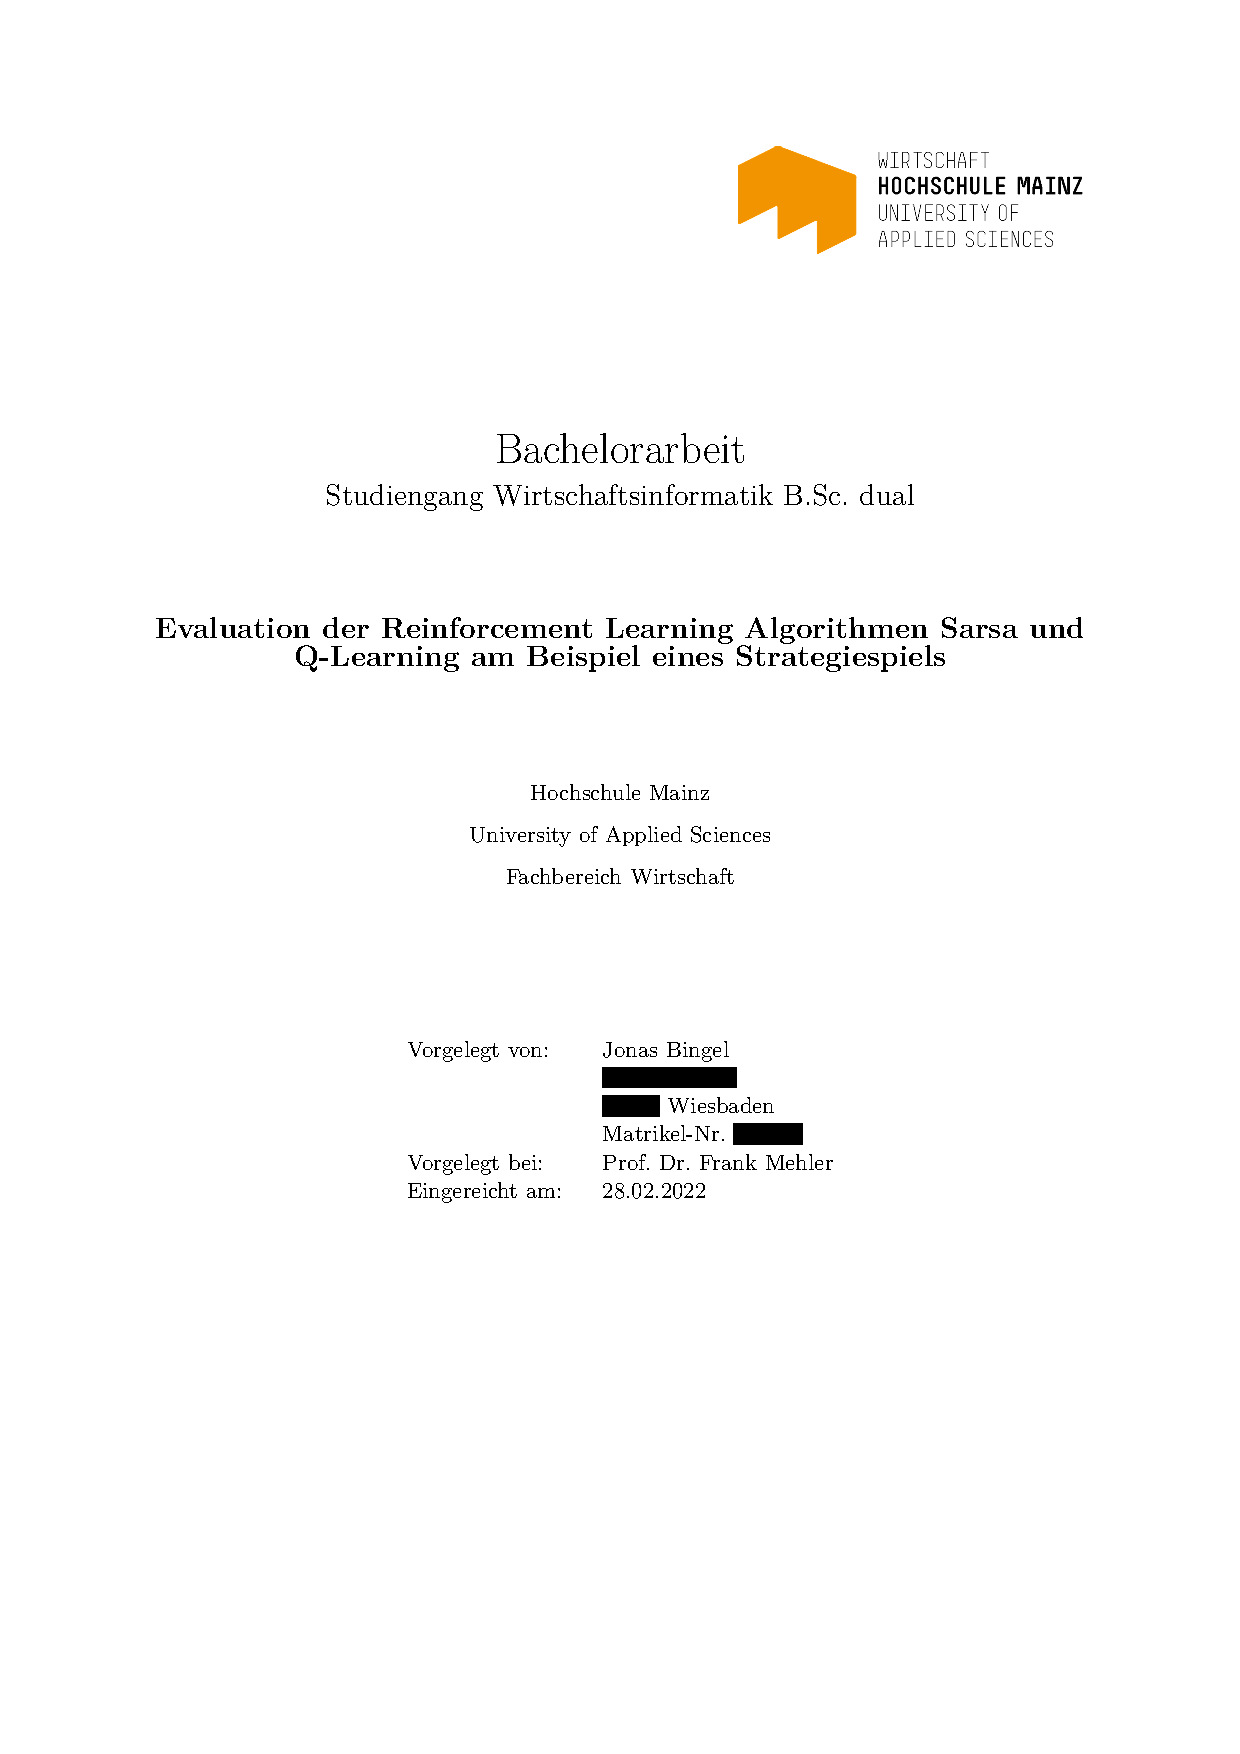
\includegraphics[width=0.7\linewidth]{04_Artefakte/BeispielPDF.pdf}}
    \caption[Beispiel für den Auszug aus einer PDF]{Beispiel für den Auszug aus einer PDF im Anhang}
\end{figure}

\chapter{Anhang Tabelle}
\label{app:longtable}
\begin{center}
\begin{longtable}{lll}
\caption{Ein Beispiel für eine lange Tabelle} \label{tab:long} \\

\toprule \multicolumn{1}{c}{\textbf{First column}} & \multicolumn{1}{c}{\textbf{Second column}} & \multicolumn{1}{c}{\textbf{Third column}} \\ \midrule 
\endfirsthead

\multicolumn{3}{c}%
{{\bfseries \tablename\ \thetable{} -- fortgesetzt von voriger Seite}} \\
\midrule \multicolumn{1}{c}{\textbf{First column}} & \multicolumn{1}{c}{\textbf{Second column}} & \multicolumn{1}{c}{\textbf{Third column}} \\ \midrule
\endhead

\midrule \multicolumn{3}{r}{{fortgesetzt auf nachfolgender Seite}} \\
\endfoot

\bottomrule
\endlastfoot
One & abcdef ghjijklmn & 123.456778 \\
One & abcdef ghjijklmn & 123.456778 \\
One & abcdef ghjijklmn & 123.456778 \\
One & abcdef ghjijklmn & 123.456778 \\
One & abcdef ghjijklmn & 123.456778 \\
One & abcdef ghjijklmn & 123.456778 \\
One & abcdef ghjijklmn & 123.456778 \\
One & abcdef ghjijklmn & 123.456778 \\
One & abcdef ghjijklmn & 123.456778 \\
One & abcdef ghjijklmn & 123.456778 \\
One & abcdef ghjijklmn & 123.456778 \\
One & abcdef ghjijklmn & 123.456778 \\
One & abcdef ghjijklmn & 123.456778 \\
One & abcdef ghjijklmn & 123.456778 \\
One & abcdef ghjijklmn & 123.456778 \\
One & abcdef ghjijklmn & 123.456778 \\
One & abcdef ghjijklmn & 123.456778 \\
One & abcdef ghjijklmn & 123.456778 \\
One & abcdef ghjijklmn & 123.456778 \\
One & abcdef ghjijklmn & 123.456778 \\
One & abcdef ghjijklmn & 123.456778 \\
One & abcdef ghjijklmn & 123.456778 \\
One & abcdef ghjijklmn & 123.456778 \\
One & abcdef ghjijklmn & 123.456778 \\
One & abcdef ghjijklmn & 123.456778 \\
One & abcdef ghjijklmn & 123.456778 \\
One & abcdef ghjijklmn & 123.456778 \\
One & abcdef ghjijklmn & 123.456778 \\
One & abcdef ghjijklmn & 123.456778 \\
One & abcdef ghjijklmn & 123.456778 \\
One & abcdef ghjijklmn & 123.456778 \\
One & abcdef ghjijklmn & 123.456778 \\
One & abcdef ghjijklmn & 123.456778 \\
One & abcdef ghjijklmn & 123.456778 \\
One & abcdef ghjijklmn & 123.456778 \\
One & abcdef ghjijklmn & 123.456778 \\
One & abcdef ghjijklmn & 123.456778 \\
One & abcdef ghjijklmn & 123.456778 \\
One & abcdef ghjijklmn & 123.456778 \\
One & abcdef ghjijklmn & 123.456778 \\
One & abcdef ghjijklmn & 123.456778 \\
One & abcdef ghjijklmn & 123.456778 \\
One & abcdef ghjijklmn & 123.456778 \\
One & abcdef ghjijklmn & 123.456778 \\
One & abcdef ghjijklmn & 123.456778 \\
One & abcdef ghjijklmn & 123.456778 \\
One & abcdef ghjijklmn & 123.456778 \\
One & abcdef ghjijklmn & 123.456778 \\
One & abcdef ghjijklmn & 123.456778 \\
One & abcdef ghjijklmn & 123.456778 \\
One & abcdef ghjijklmn & 123.456778 \\
One & abcdef ghjijklmn & 123.456778 \\
One & abcdef ghjijklmn & 123.456778 \\
One & abcdef ghjijklmn & 123.456778 \\
One & abcdef ghjijklmn & 123.456778 \\
One & abcdef ghjijklmn & 123.456778 \\
One & abcdef ghjijklmn & 123.456778 \\
One & abcdef ghjijklmn & 123.456778 \\
One & abcdef ghjijklmn & 123.456778 \\
One & abcdef ghjijklmn & 123.456778 \\
One & abcdef ghjijklmn & 123.456778 \\
One & abcdef ghjijklmn & 123.456778 \\
One & abcdef ghjijklmn & 123.456778 \\
One & abcdef ghjijklmn & 123.456778 \\
One & abcdef ghjijklmn & 123.456778 \\
One & abcdef ghjijklmn & 123.456778 \\
One & abcdef ghjijklmn & 123.456778 \\
One & abcdef ghjijklmn & 123.456778 \\
One & abcdef ghjijklmn & 123.456778 \\
One & abcdef ghjijklmn & 123.456778 \\
One & abcdef ghjijklmn & 123.456778 \\
One & abcdef ghjijklmn & 123.456778 \\
One & abcdef ghjijklmn & 123.456778 \\
One & abcdef ghjijklmn & 123.456778 \\
One & abcdef ghjijklmn & 123.456778 \\
\end{longtable}
\end{center}


\usestandardtocs
\bookmarksetup{startatroot}% siehe bookmark-Anleitung

\end{document}
